\documentclass{beamer}
\usepackage{amsmath,amsbsy,amsopn,amstext,amsfonts,amssymb}
\usepackage{isomath}
\usepackage{ulem}
%\linespread{1.6}  % double spaces lines
\usepackage{graphicx}
\usepackage{subfigure}
\usepackage{color}
\usepackage{optidef}  % define optimization problems
\usepackage{multicol}  % multiple columns
\usepackage{listings} % for python code
\usepackage{mathrsfs}

\usepackage{polynom}
\newcommand{\adj}{\mathrm{adj}}
\newcommand{\constrainedmin}[3]{
		\begin{mini*}|s|
		{#2}{#1}{}{}
		\addConstraint{#3}
		\end{mini*}
}

\newcommand{\rwbcomment}[1]{{\color{blue}RWB:#1}}
\newcommand{\defeq}{\stackrel{\triangle}{=}}
\newcommand{\abs}[1]{\left|#1\right|}
\newcommand{\norm}[1]{\left\|#1\right\|}
\newcommand{\iprod}[1]{\left<#1\right>}
\newcommand{\ellbf}{\boldsymbol{\ell}}
\newcommand{\nubf}{\boldsymbol{\nu}}
\newcommand{\mubf}{\boldsymbol{\mu}}
\newcommand{\abf}{\mathbf{a}}
\newcommand{\bbf}{\mathbf{b}}
\newcommand{\cbf}{\mathbf{c}}
\newcommand{\dbf}{\mathbf{d}}
\newcommand{\ebf}{\mathbf{e}}
\newcommand{\fbf}{\mathbf{f}}
\newcommand{\gbf}{\mathbf{g}}
\newcommand{\hbf}{\mathbf{h}}
\newcommand{\ibf}{\mathbf{i}}
\newcommand{\jbf}{\mathbf{j}}
\newcommand{\kbf}{\mathbf{k}}
\newcommand{\lbf}{\mathbf{l}}
\newcommand{\mbf}{\mathbf{m}}
\newcommand{\nbf}{\mathbf{n}}
\newcommand{\obf}{\mathbf{o}}
\newcommand{\pbf}{\mathbf{p}}
\newcommand{\qbf}{\mathbf{q}}
\newcommand{\rbf}{\mathbf{r}}
\newcommand{\sbf}{\mathbf{s}}
\newcommand{\tbf}{\mathbf{t}}
\newcommand{\ubf}{\mathbf{u}}
\newcommand{\vbf}{\mathbf{v}}
\newcommand{\wbf}{\mathbf{w}}
\newcommand{\xbf}{\mathbf{x}}
\newcommand{\ybf}{\mathbf{y}}
\newcommand{\zbf}{\mathbf{z}}
\newcommand{\Jbf}{\mathbf{J}}
\newcommand{\Acal}{\mathcal{A}}
\newcommand{\Bcal}{\mathcal{B}}
\newcommand{\Lcal}{\mathcal{L}}
\newcommand{\Ncal}{\mathcal{N}}
\newcommand{\Rcal}{\mathcal{R}}
\definecolor{darkolivegreen}{rgb}{0.33, 0.42, 0.18}

\makeatletter
\newenvironment<>{proofstart}[1][\proofname]{%
    \par
    \def\insertproofname{#1\@addpunct{.}}%
    \usebeamertemplate{proof begin}#2}
  {\usebeamertemplate{proof end}}
\newenvironment<>{proofcont}{%
  \setbeamertemplate{proof begin}{\begin{block}{}}
    \par
    \usebeamertemplate{proof begin}}
  {\usebeamertemplate{proof end}}
\newenvironment<>{proofend}{%
    \par
    \pushQED{\qed}
    \setbeamertemplate{proof begin}{\begin{block}{}}
    \usebeamertemplate{proof begin}}
  {\popQED\usebeamertemplate{proof end}}
\makeatother

\title{ECEn 671: Mathematics of Signals and Systems}
\author{Randal W. Beard}
\institute{Brigham Young University}
\date{\today}

\begin{document}

%-------------------------------
\begin{frame}
	\titlepage
\end{frame}




%%%%%%%%%%%%%%%%%%%%%%%%%%%%%%%%%%%%%%%%%%%%%%%%%%%%%%%%%%%%%%%%%%%%%%%
\section{Gram Schmidt Orthogonalization}
\frame{\sectionpage}


%----------------------------------
\begin{frame}\frametitle{Application:  Gram Schmidt Orthogonalization}
\noindent Given a set $T = \{ p_1, \ldots, p_n\}$

\noindent Find a set $T' = \{q_1, \ldots, q_n'\} \qquad n' \leq n$ such that
\[ span(T') = span(T) \text{ and } <q_i,q_j> = \delta_{ij} \]

\begin{description}
\item[Step 1.]
Normalize the First Vector
\[ q_1 = \frac{p_1}{\norm{ p_1 }} \qquad \text{ (i.e. } \iprod{ q_1,q_1 }=1 \text{ ) } \]
\end{description}
\end{frame}

%----------------------------------
\begin{frame}\frametitle{Application:  Gram Schmidt Orthogonalization, cont}

\begin{description}
\item[Step 2.]	
Let $e_2$ be $p_2$ minus the projection of $p_2$ on $q_1$
i.e.
\[ e_2 = p_2 - \iprod{ p_2, q_1} q_1 \]

\begin{center}
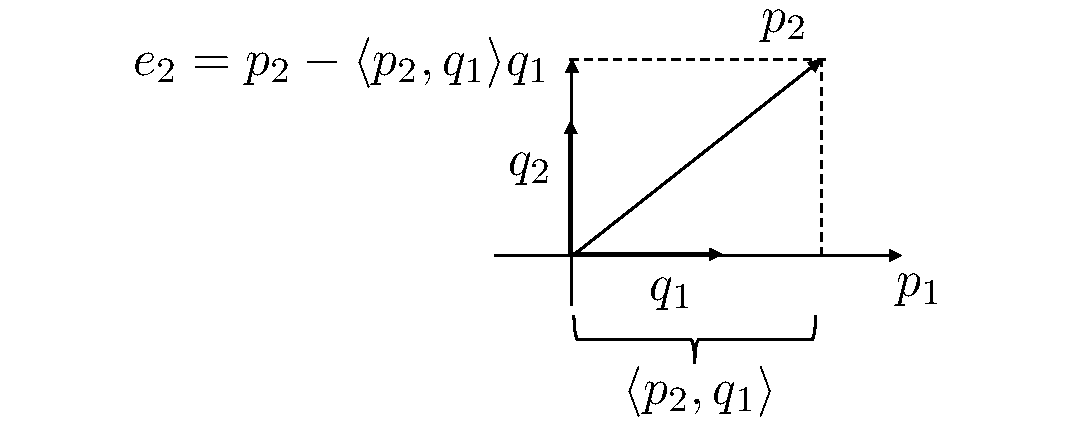
\includegraphics[width=4in]{figures/chap2_gram_schmidt}
\end{center}

Then normalize $e_2$:
\[ q_2 = \frac{e_2}{\norm{ e_2 }} \]
\end{description}
\end{frame}

%----------------------------------
\begin{frame}\frametitle{Application:  Gram Schmidt Orthogonalization, cont}

\begin{description}
\item[Step 3.]
Let $e_k$ be $p_k$ minus the projection of $p_k$ on $q_1, \ldots, q_{k-1}$:
\[ e_k = p_k - \sum_{j=1}^{k-1}\iprod{ p_k, q_j} q_j \Rightarrow q_k = \frac{e_k}{\norm{ e_k }} \]
\end{description}
\end{frame}

%----------------------------------
\begin{frame}\frametitle{Example: Gram Schmidt Orthogonalization}
Given the set
\[
T = \{ p_1, p_2, p_3 \} \defeq \left\{ \begin{pmatrix} 2 \\ 0 \\ 0 \end{pmatrix}, \begin{pmatrix}1 \\ 2 \\ 0 \end{pmatrix}, \begin{pmatrix} 1 \\ 2 \\ 3 \end{pmatrix} \right\}
\]	
find a set $T'=\{q_1, q_2, q_3\}$ where the vectors in $T'$ are orthonormal and $\text{span}(T)=\text{span}(T')$.

\vfill

\[
q_1 = \frac{p_1}{\norm{p_2}} = \frac{\begin{pmatrix} 2 \\ 0 \\ 0 \end{pmatrix}}{2} = \begin{pmatrix} 1 \\ 0 \\ 0 \end{pmatrix}.
\]

\end{frame}

%----------------------------------
\begin{frame}\frametitle{Example: Gram Schmidt Orthogonalization, cont.}

\begin{align*}
e_2 &= p_2 - \iprod{p_2, q_1} q_1 \\
    &= \begin{pmatrix} 1 \\ 2 \\ 0 \end{pmatrix} - \begin{pmatrix} 1\\2\\0\end{pmatrix}^\top\begin{pmatrix}1\\0\\0\end{pmatrix}\begin{pmatrix}1\\0\\0\end{pmatrix} \\
    &= \begin{pmatrix} 1 \\ 2 \\ 0 \end{pmatrix} - 1\cdot\begin{pmatrix}1\\0\\0\end{pmatrix} \\
    &= \begin{pmatrix}0\\2\\0\end{pmatrix}
\end{align*}
Therefore
\(
q_2 = \frac{e_2}{\norm{e_2}} = \frac{\begin{pmatrix}0\\2\\0\end{pmatrix}}{2} = \begin{pmatrix}0\\1\\0\end{pmatrix}
\)

\end{frame}

%----------------------------------
\begin{frame}\frametitle{Example: Gram Schmidt Orthogonalization, cont.}

\begin{align*}
e_3 &= p_3 - \iprod{p_3, q_1} q_1 -\iprod{p_3, q_2}q_2 \\
    &= \begin{pmatrix} 1 \\ 2 \\ 3 \end{pmatrix} - \begin{pmatrix} 1\\2\\3\end{pmatrix}^\top\begin{pmatrix}1\\0\\0\end{pmatrix}\begin{pmatrix}1\\0\\0\end{pmatrix} - \begin{pmatrix} 1\\2\\3\end{pmatrix}^\top\begin{pmatrix}0\\1\\0\end{pmatrix}\begin{pmatrix}0\\1\\0\end{pmatrix} \\
    &= \begin{pmatrix} 1 \\ 2 \\ 3 \end{pmatrix} - 1\cdot\begin{pmatrix}1\\0\\0\end{pmatrix}  - 2\cdot\begin{pmatrix}0\\1\\0\end{pmatrix} \\
    &= \begin{pmatrix}0\\0\\3\end{pmatrix}
\end{align*}
Therefore
\(
q_3 = \frac{e_3}{\norm{e_3}} = \frac{\begin{pmatrix}0\\0\\3\end{pmatrix}}{3} = \begin{pmatrix}0\\0\\1\end{pmatrix}
\)

\end{frame}

%----------------------------------
\begin{frame}\frametitle{Example: Gram Schmidt Orthogonalization, cont.}

Therefore, the Gram Schmidt orthonormalization of 
\[
T = \{ p_1, p_2, p_3 \} \defeq \left\{ \begin{pmatrix} 2 \\ 0 \\ 0 \end{pmatrix}, \begin{pmatrix}1 \\ 2 \\ 0 \end{pmatrix}, \begin{pmatrix} 1 \\ 2 \\ 3 \end{pmatrix} \right\}
\]	
is
\[
T' = \{q_1, q_2, q_3\} = \left\{ \begin{pmatrix} 1 \\ 0 \\ 0 \end{pmatrix}, \begin{pmatrix}0 \\ 1 \\ 0 \end{pmatrix}, \begin{pmatrix} 0 \\ 0 \\ 1 \end{pmatrix} \right\}.
\]

\vfill

Note that $\text{span}(T)=\text{span}(T')$.

\end{frame}




\end{document}